%%%%%%%%%%%%%%%%%%%%%%%%%%%%%%%%%%%%%%%%%%%%%%%%%%%%%%%%%%%%%%%%%%%%%%
%%                     absolute stimulation
%%%%%%%%%%%%%%%%%%%%%%%%%%%%%%%%%%%%%%%%%%%%%%%%%%%%%%%%%%%%%%%%%%%%%%
\color{ForestGreen}

\subsubsection{Glyph: \glyph{Absolute inhibition}}\label{sec:absoluteInhibition}

An \glyph{absolute inhibition} precludes the existence of another relationship. A relationship modulated by an absolute inhibition can only exist when an absolute inhibition in false, whatever are the other influences this relationship is subjected to.

\begin{glyphDescription}
 \glyphSboTerm SBO:0000407 ! absolute inhibition.
 \glyphOrigin Any \glyph{entity node} (\sect{ENs}).
 \glyphTarget Any \glyph{relationship} (\sect{relationships}).
 \glyphEndPoint The target extremity of a \glyph{absolute inhibition} carries a double bar perpendicular to the arc (to remind that it is an \glyph{inhibition}).
\begin{itemize}
\item the \glyph{entity node} from which the influence targeted by the \glyph{absolute inhibition} origins
\item all the relevant \glyph{interactors} of the \glyph{interaction} or the \glyph{non-interaction} targeted by the \glyph{absolute inhibition}
\item the \glyph{entity} subjected to the \glyph{assignment} targeted by the \glyph{absolute inhibition}
\end{itemize}

 \end{glyphDescription}

\begin{figure}[H]
  \centering
  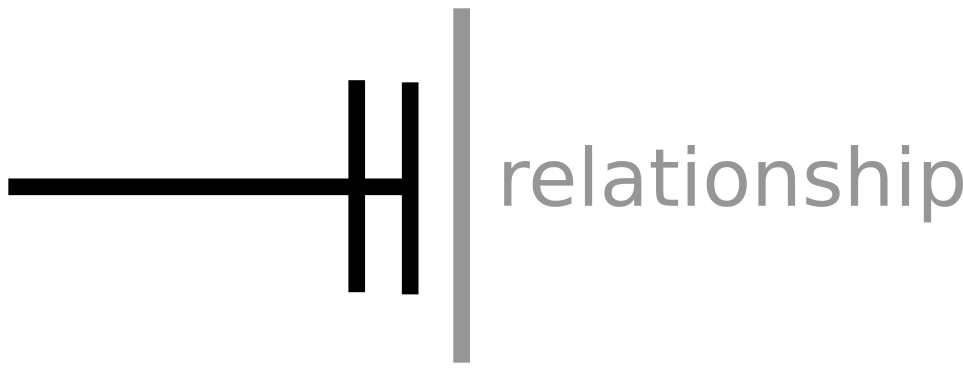
\includegraphics[scale = 0.5]{images/absoluteInhibition}
  \caption{The \PD glyph for \glyph{absoluteInhibition}.}
  \label{fig:absoluteInhibition}
\end{figure}

\begin{figure}[H]
  \centering
  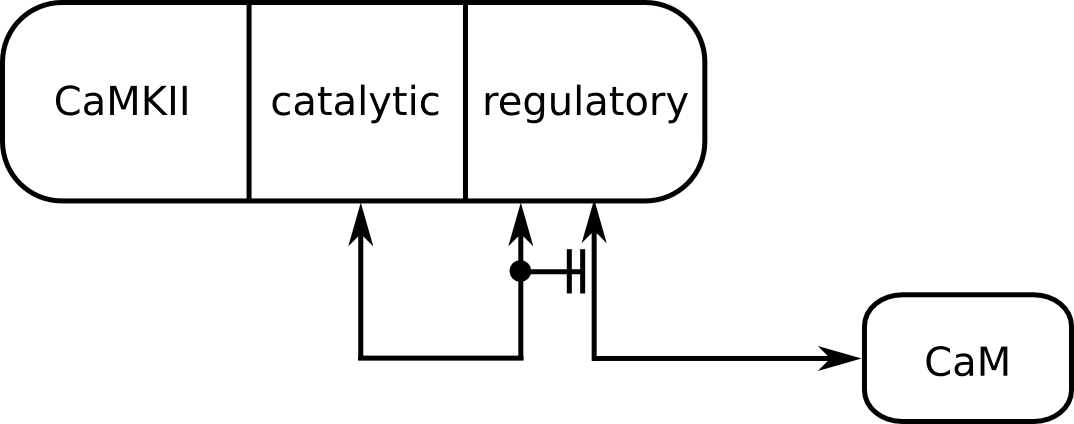
\includegraphics[scale = 0.5]{examples/ex-absoluteInhibition}
  \caption{This example shows how an intra-molecular interaction of CaMKII precludes totally its catalytic activity upon another molecule of CaMKII.}
  \label{fig:ex-absoluteInhibition}
\end{figure}

\normalcolor